\documentclass{ieeeaccess}%
\usepackage{cite}
\usepackage{amsmath,amssymb,amsfonts}
\usepackage{algorithmic}
\usepackage{graphicx}
\usepackage{textcomp}
\usepackage{caption}
\usepackage{subcaption}
\usepackage{float}
\usepackage[flushleft]{threeparttable}
\usepackage{amsmath}
\usepackage{amsfonts}
\usepackage{amssymb}%
\setcounter{MaxMatrixCols}{30}
%TCIDATA{OutputFilter=latex2.dll}
%TCIDATA{Version=5.50.0.2960}
%TCIDATA{LastRevised=Tuesday, November 16, 2021 16:02:39}
%TCIDATA{<META NAME="GraphicsSave" CONTENT="32">}
%TCIDATA{<META NAME="SaveForMode" CONTENT="1">}
%TCIDATA{BibliographyScheme=Manual}
%BeginMSIPreambleData
\providecommand{\U}[1]{\protect\rule{.1in}{.1in}}
%EndMSIPreambleData
\newtheorem{theorem}{Theorem}
\newtheorem{acknowledgement}[theorem]{Acknowledgement}
\newtheorem{algorithm}[theorem]{Algorithm}
\newtheorem{axiom}[theorem]{Axiom}
\newtheorem{case}[theorem]{Case}
\newtheorem{claim}[theorem]{Claim}
\newtheorem{conclusion}[theorem]{Conclusion}
\newtheorem{condition}[theorem]{Condition}
\newtheorem{conjecture}[theorem]{Conjecture}
\newtheorem{corollary}[theorem]{Corollary}
\newtheorem{criterion}[theorem]{Criterion}
\newtheorem{definition}[theorem]{Definition}
\newtheorem{example}[theorem]{Example}
\newtheorem{exercise}[theorem]{Exercise}
\newtheorem{lemma}{Lemma}
\newtheorem{notation}{Notation}
\newtheorem{problem}[theorem]{Problem}
\newtheorem{proposition}[theorem]{Proposition}
\newtheorem{remark}{Remark}
\newtheorem{solution}[theorem]{Solution}
\newtheorem{summary}[theorem]{Summary}
\newenvironment{proof}[1][Proof]{\noindent\textbf{#1.} }{\ \rule{0.5em}{0.5em}}
\def\BibTeX{{\rm B\kern-.05em{\sc i\kern-.025em b}\kern-.08em
    T\kern-.1667em\lower.7ex\hbox{E}\kern-.125emX}}

\begin{document}

\title{Title}
\author{\uppercase{Bor-Sen Chen}\authorrefmark{1,2}, \IEEEmembership{Life
Fellow, IEEE}, \uppercase{Ting-Wei Hung\authorrefmark{1}}}

\begin{abstract}
$H_{\infty}$
\end{abstract}

\begin{keywords}
keywords
\end{keywords}

\history{Date of publication xxxx 00, 0000, date of current version xxxx 00,
0000.} \doi{doi}

\address[1]{Department of Electrical Engineering, National Tsing Hua
University, Hsinchu 30013, Taiwan} \address[2]{Department of Electrical
Engineering, Yuan Ze University, Taoyuan 32003, Taiwan}

\tfootnote{This work was supported by the Ministry of Science and Technology
of Taiwan under Grant MOST 108-2221-E-007-099-MY3.}

\markboth
{Author \headeretal: Title}
{Author \headeretal: Title}

\corresp{Corresponding author: Bor-Sen Chen (bschen@ee.nthu.edu.tw)} \titlepgskip=-15pt
\maketitle

\section{INTRODUCTION}

\PARstart{W}{ith} test cite 1 \cite{gait1}.

The contributions of this study are described as follows:

\begin{enumerate}
\item contribution 1

\item contribution 2

\end{enumerate}

\ The study is organized as follows. In Section II, ...

\textbf{Notation 1:} 

% bold font
\textbf{Notation 2:} 

\section{PRELIMINARIES OF UAV AND BIPED ROBOT}

In this study, ...

\subsection{UAV}

\begin{figure}[htbp]
\centering
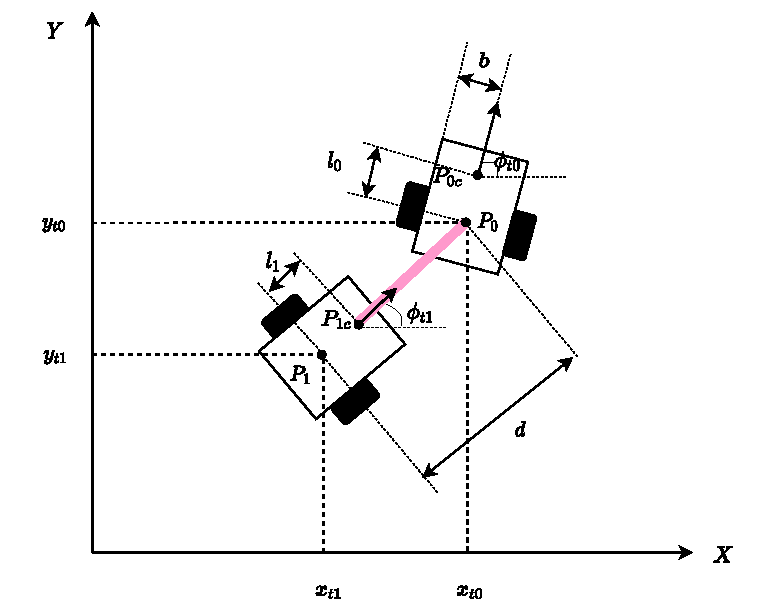
\includegraphics[width=0.43\textwidth]{tractor-trailer.pdf}
\caption{tractor-trailer test}%
\label{fig:tractor-trailer}%
\end{figure}

% italics
\textit{Assumption II.A.1:} Assumption

\textit{Assumption II.A.2:} The inertia matrix $M_{t}(\cdot)$ 

% equation
\begin{equation}
X_{t}(t)=[x_{t,1}(t)\text{ }y_{t,1}(t)\text{ }\phi_{t,1}(t)\text{ }\phi
_{t,0}(t)]^{T}
\label{tt state-space x}
\end{equation}

% align
\begin{align}
&  A_{t}(X_{t}(t))\dot{X}_{t}(t)\label{tt constraint Adx=0}\\
&  =\left[
\begin{array}
[c]{ll}%
\sin\phi_{t,0}(t) & \sin\phi_{t,1}(t)\\
-\cos\phi_{t,0}(t) & -\cos\phi_{t,1}(t)\\
-d\cos(\phi_{t,0}(t)-\phi_{t,1}(t)) & 0\\
0 & 0
\end{array}
\right]  ^{T}\nonumber\\
&
\begin{array}
[c]{l}%
\times\left[
\begin{array}
[c]{l}%
\dot{x}_{t,1}(t)\\
\dot{y}_{t,1}(t)\\
\dot{\phi}_{t,1}(t)\\
\dot{\phi}_{t,0}(t)
\end{array}
\right]  =0
\end{array}
\nonumber
\end{align}

\begin{remark}
remark test
\end{remark}

% lemma
\begin{lemma}
(\cite{lemma}) For any matrix $X$ and $Y$ with appropriate dimensions, the
following inequality holds:%
\begin{equation}
X^{T}Y+Y^{T}X\leq X^{T}P^{-1}X+Y^{T}PY \label{lemma inequality}%
\end{equation}
where $P$ is any positive definite symmetric matrix.
\end{lemma}

% theorem
\begin{theorem}
therom test
\end{theorem}

\begin{proof}
proof test
\end{proof}


\EOD

\end{document}